\chapter{Appendix}\label{apx:appendix}

\section{FlexSight Project}\label{apx:flexsight}
One of the key challenges in most robotics applications, from robot­aided manufacturing to service robotics applications, is the capability to automatically identify and locate various types of objects, in such a way that the robot can grasp and manipulate them accurately and reliably.

Depending on the application, objects can be regularly disposed in trays, but often they are randomly placed inside bins, or over tables, pallets or conveyor belts. A reliable perception systems is thus required to identify and precisely locate the objects, and to guide robots during the manipulation tasks. Due to the strong impact of these systems in terms of productivity, they have been widely studied in the last decades. Nowadays, many products have been proposed to solve this problem that, under a scientific point of view, it can be considered a very mature topic. Still, almost all the implemented systems assume to deal with rigid, non-deformable objects; moreover, they often assume that object instances of a given object class (e.g., a package)  have all the same size and the same form factor.

FlexSight aims to remove these limiting assumptions, by proposing a perception system that is also able to recognize and localize several types of deformable objects that can be commonly found in many industrial and logistic applications, such as soft sacks, deformable and variable size packaging, food products, articles of clothing, flexible assembly parts, etc ... 
As \emph{deformable objects} (See \figref{fig:deformable_objects_ex}) are intended either as an object that can change its shape or dimensions due to a stress or, with an abuse of notation, as each object that can be obtained from a basic template by applying a resize operator along one or more directions (e.g., a cubic parcel post can be conceptually \emph{deformed} in many kind of parcel posts).

\begin{figure}
    \centering
    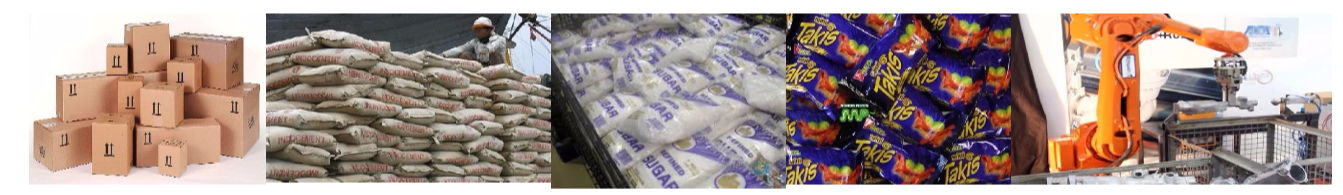
\includegraphics[width=\textwidth]{figures/Appendix/deformable_objects_ex.png}
    \caption{\textbf{Examples of deformable objects}. As deformable objects are intended either as objects that can change their shape or dimensions due to a stress or, with an abuse of notation, as each object that can be obtained from a basic template by applying a resize operator along one or more directions (e.g., a cubic parcel post can be conceptually deformed in many kind of parcel posts).} 
    \label{fig:deformable_objects_ex}
\end{figure}

The main objectives of the FlexSight experiment are:

\begin{itemize}
	\item Enable a robot to perceive a large and widespread class of rigid and deformable objects in an accurate and reliable way, with a particular emphasis on the computational speed of the whole system;
	\item Implement a prototype of a compact industrial sensor (the FlexSight Sensor, FSS for brevity), that integrates inside a robust and small chassis all the required sensors and a processing unit suitable to run the detection and localization algorithms. Our aim is to provide the robot integrators with a sensor that can be easily fitted into conventional robotics cells, thus enabling fully automated and unsupervised procedures in new areas, where usually the intervention of an operator for handling operations is required;
	\item Integrate the FlexSight Sensor inside a working system that will be tested in several industrial and logistic use cases.
\end{itemize}

\subsection{Progress beyond the current state of the technology}\label{subsec:flexsight_related_works}
A wide range of industrial products are packaged in soft bags, sacks or soft packagings. The handling and the palletization of such items during the production is addressed with well engineered and repeatable processes. This is not the case for the industrial end user of these products: they are often randomly placed inside bins or over pallets, so pick\&place operations are performed with forklifts, hoists and/or cranes driven by an operator, leading to significant drawbacks, including health issues (toxic material), hygiene (e.g., in food industry) and efficiency of manual operation. On the other hand, the task of automatically sorting small packages with variable and deformable shapes (e.g., food packages, parcel posts, etc…) inside unstructured environments still remains a challenging problem. A robotic system that can automatically identify, locate, grasp and manipulate all these types of deformable objects is therefore highly desirable.

Many industrial robotics pick\&place systems have been studied and proposed in the last decades. Typically: (1) Either these systems assume to deal with rigid, non deformable objects, where an exact CAD model of the searched objects is provided, or (2) they assume to deal with slightly different instances of the same object class (as in the case of fruits), but objects are placed on a plane or on a conveyor belt and they are isolated, thus making the identification and manipulation relatively easy. Within the FlexSight experiment, we aim to overcome these assumptions. The challenge is first of all technological: even if there is a relevant body of scientific papers dealing with this topic, in most cases they are designed for different purposes (e.g., object categorization) or they are proof of concepts, that is they do not consider the challenges arising in bringing these technologies in highly reliable, industrial environment, that will be addressed below.

Most of the current pick\&place systems employ a recognition and localization system based on vision, 3D depth sensors or RGB-D cameras. They typically employ a standard pipeline of processing blocks:

\begin{figure}[!hbt]
    \centering
    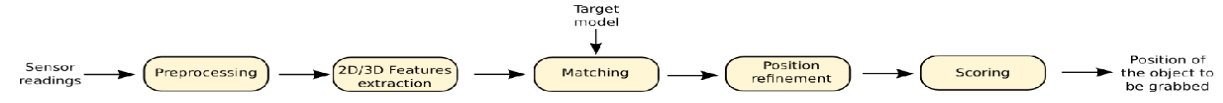
\includegraphics[width=\textwidth]{figures/Appendix/flex_1.png} 
    \label{fig:flex_1}
\end{figure}

Sub-sampling, clustering and noise reduction are often used in the preprocessing blocks, while 2D and/or 3D descriptors are widely used in current systems. The matching block usually aims to associate the extracted features with features pre-computed from a rigid template (e.g., the CAD model) of the object, sample consensus methods are widely used in this case. The result is a set of object candidates, that is refined using iterative optimization strategy (e.g., Iterative Closest Point).

Many research works overcome the assumption of the rigid template model, by proposing several models and techniques to deal with deformable objects but they actually, devoted little effort to develop and test industrial systems able to accurately recognize and localize in 3D, highly deformable and variable objects. In the FlexSight experiment we aim to overcome most of these limitations, enabling an effective \emph{from lab to market} technology transfer: we will investigate among the most promising 3D object modeling solutions, designing an automatic procedure that acquires a multiple-template deformation model (target multi-model) of the objects. The recognition procedure will extract a set of object hypotheses using model-based, visual and 3D structure cues, matched with the target multi-model. Position refinement will be obtained with an efficient optimization procedure that estimates both the position and the deformation parameters of each candidate. Leveraging on the perception outputs, the grasping and manipulation modules will be designed using state of the art hardware and software solutions, enabling reliable and efficient pick\&place operations.

%\section{RoboCup@Work}\label{apx:robocupatwork}
%To do ...